\documentclass[twocolumn, a4paper]{article}

\usepackage{amsthm, amsmath, amssymb}
\usepackage{microtype}
\usepackage{graphicx}
\usepackage{booktabs} % for professional tables
\usepackage{hyperref}
\usepackage{multirow}
\urlstyle{same}
\hypersetup{colorlinks=true, linkcolor=black, citecolor=black, urlcolor=blue}

\usepackage{subcaption}

\usepackage[top=2cm, bottom=2cm, left=1.5cm, right=1.5cm]{geometry}
\usepackage{titlesec}
    \titleformat{\title}{\large\bfseries}{}{}{}
    \titleformat{\section}{\normalfont\bfseries}{\thesection}{0.5em}{}
    \titleformat{\subsection}{\normalfont\it}{\thesubsection}{0.5em}{}
    \titleformat{\subsubsection}{\normalfont\normalsize\it}{\thesubsubsection}{0.5em}{}
    \titleformat{\paragraph}[runin]{\normalfont\bfseries}{\theparagraph}{0.5em}{}
    \titleformat{\subparagraph}[runin]{\normalfont\normalsize\it}{\thesubparagraph}{0.5em}{}
\usepackage[font=small,labelfont=bf,labelsep=space]{caption}

% \usepackage[ruled]{algorithm2e}
% \SetKwComment{Comment}{// }{ }

\usepackage{graphicx}
\graphicspath{{../assets}}

\usepackage{tikz}
% \usetikzlibrary{shapes.geometric, arrows}
% \usetikzlibrary{calc}

% \tikzstyle{main_node} = [circle, minimum width=1cm,text centered, draw=black, fill=red!30]
% \tikzstyle{neigh_node} = [circle, minimum width=1cm,text centered, draw=black, fill=green!30]
% \tikzstyle{node} = [circle, minimum width=1cm,text centered, draw=black, fill=cyan!30]
% \tikzstyle{arrow} = [thick,->,>=stealth]

\usepackage{pgfplots}
\pgfplotsset{compat=1.18}

\pgfplotsset{
    report_style/.style={
    legend style={draw=none, font=\small},
    legend cell align=left,
    legend pos=north east,
    ylabel style={align=center, font=\bfseries\boldmath},
    xlabel style={align=center, font=\bfseries\boldmath},
    x tick label style={font=\bfseries\boldmath},
    y tick label style={font=\bfseries\boldmath},
    scaled ticks=false,
    every axis plot/.append style={thick},
    },
}

\newtheorem{theorem}{Theorem}
\newtheorem{lemma}{Lemma}
\newtheorem{corollary}{Corollary}
\theoremstyle{definition}
\newtheorem{definition}{Definition}

\begin{document}

\title{\bf\Large Segmentation of 3D volume images for connectomics}
\author{Oleh Shkalikov\texorpdfstring{ (5102818)
\\[0.7em]{\small Supervisors: Jannik Irmai, David Stein}
\\{\small Chairholder: Prof. Dr. Bjoern Andres}}{}}
\date{CMS Research project, TU Dresden}

\twocolumn[
    \begin{@twocolumnfalse}
        \maketitle

        \vspace{7ex}
    \end{@twocolumnfalse}
]

\section{Introduction}
The aim of this research project is to develop approaches
for segmentation of 3D volume images for connectomics given
a labeled dataset. The importance of this problem comes from the
developing of methods (e.g. \cite{10.7554/eLife.25916}) of acquiring high resolution volume images
which makes hard to analyze all gathered data by hand because of their size.
Therefore automatic methods such as automatic labeling of data is needed.

In this work we will propose CNN based methods for solving this task and evaluate them
on the given dataset.

\section{Dataset description and analysis} \label{sec:data_analysis}

The labeled dataset which we use for out project is based on
the image volumes of the CA1 hippocampus region of the brain
acquired by a focused ion beam scanning electron microscope (FIB-SEM).
The raw data has a shape \( 2048 \times 1536 \times 1065 \)  and is available under
\url{https://www.epfl.ch/labs/cvlab/data/data-em/}. It was initially used in
\cite{lucchi2011supervoxel,lucchi2013learning} because this dataset also contains binary
labels for mitochondria which we don't use because we have been provided with wider
set of labels. The given connectomics volume image of the brain is
isotropic which allow us to rotate the volume/subvolumes without any side effects.

The actual labeling has been performed by An Dang Thanh (student of the MLCV lab)
only on slices of subvolumes where to
each pixel of slice \textbf{one} of the following labels has been assigned:
\begin{enumerate}
    \itemsep0em
    \item cell cytoplasm
    \item cell membrane
    \item mitochondrion
    \item mitochondrion membrane
    \item synapse
    \item vesicle
    \item undefined (in the case where annotator was uncertain about the correct label)
\end{enumerate}
In total 9 slices of the raw data volume has been labeled and split into train,
validation and test splits: 3 slices for each split, but every train slice has a shape
\( 600 \times 600 \) whereas every validation and test slice has a shape \( 425 \times 425 \).
The locations of slices in the raw volume are denoted in the table~\ref{tab:data_loc}.
\begin{table}[t]
    \centering
    \begin{tabular}{c|c|c|c}
        Split                             & X range            & Y range            & Z range           \\
        \hline

        \multirow[vpos]{3}{*}{Train}      & \( [510, 1109] \)  & \( [200, 799] \)   & 200               \\
                                          & \( [510, 1109] \)  & 510                & \( [150, 749 ] \) \\
                                          & \( 595  \)         & \( [200, 799] \)   & \( [150, 749 ] \) \\
        \hline
        \multirow[vpos]{3}{*}{Validation} & \( [675, 1099] \)  & \( [1000, 1424] \) & 320               \\
                                          & \( [675, 1099] \)  & 1140               & \( [200, 624] \)  \\
                                          & \( 985  \)         & \( [1000, 1424] \) & \( [200, 624] \)  \\
        \hline
        \multirow[vpos]{3}{*}{Test}       & \( [1325, 1749] \) & \( [1000, 1424] \) & 650               \\
                                          & \( [1325, 1749] \) & 1100               & \( [350, 774 ] \) \\
                                          & \( 1532  \)        & \( [1000, 1424] \) & \( [350, 774 ] \) \\
        \hline
    \end{tabular}
    \caption{Location of the labeled slices in the raw volume}
    \label{tab:data_loc}
\end{table}

The dataset has been labeled by a non bio-medical expert, therefore there is a chance of mistakes
in the labeling. Another limitation of the dataset is the fact that the same pixel can represent
different biological structures and therefor labels whereas in our dataset we have only one label for
every pixel. For example, vesicles and mitochondria are part of the cell cytoplasm or
synapses are labeled as regions where a neuron passes a signal to another neuron and belong
to cell membranes and cell cytoplasm.

\begin{figure}[ht]
    \centering
    \begin{tikzpicture}
        \begin{axis}[
                report_style,
                ybar,
                xlabel={Class label},
                ylabel={Number of pixels},
                small
            ]
            \addplot+[] table[x=label,y=counts, col sep=comma] {../data/label_dist.csv};
        \end{axis}
    \end{tikzpicture}
    \caption{The distribution of labels for the train split}
    \label{fig:dist_labels}
\end{figure}

\begin{figure*}[t]
    \begin{subfigure}{0.49 \textwidth}
        \centering
        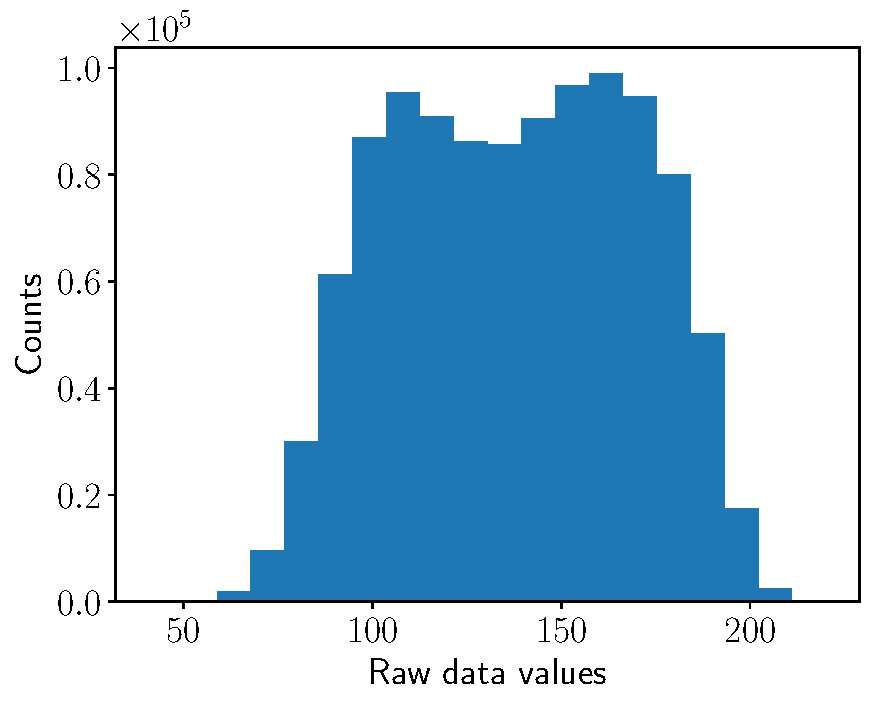
\includegraphics[width=0.85\textwidth]{raw_data_dist.pdf}
        \caption{all labels}
    \end{subfigure}
    \begin{subfigure}{0.49 \textwidth}
        \centering
        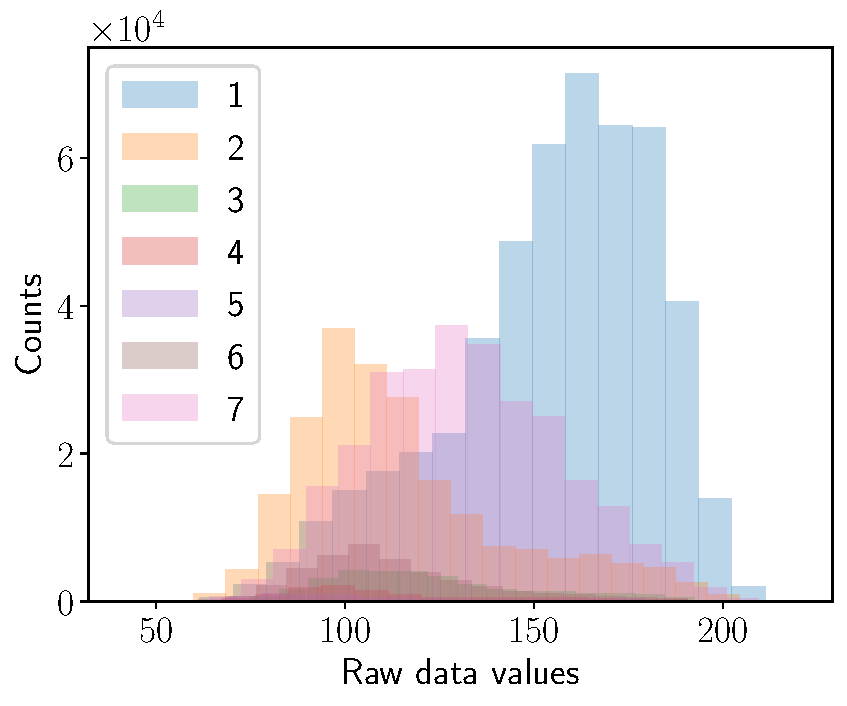
\includegraphics[width=0.85\textwidth]{raw_data_dist_per_label.pdf}
        \caption{grouped by label}
    \end{subfigure}
    \caption{The distribution of raw data for train split}
    \label{fig:dist_raw_train}
\end{figure*}

Data have a property of a high class imbalance, in particular: 46\% of all training data belongs to
cell cytoplasm, 19.4 \% to cell membrane and the remaining to other labels.
Also it worth to mention that 25.8 \% of the training split is not labeled
(i.e. label undefined has been assigned) and usually non labeled regions corresponds to
the places where several labels are adjacent and it is not clear to which class pixel should belongs to.
Therefore the hardest regions of the volume are not labeled and it can affect the performance of models
trained on this data since we use an inductive learning approach.
The distribution of the class labels for the train split is depicted on figure \ref{fig:dist_labels}.

Then we analyzed the distribution of raw data values for the train split. The histograms
are shown on figure \ref{fig:dist_raw_train}. Based on the fact that data look like it has
a normal distribution the results of statistical test of normality \cite{normalitytest} with a
null hypothesis that data is normally distributed have shown that data are not normally distributed
(all p values less than \( 10^{-182} \)) with very high confidence level.

Another important question which can be answered from data is whether means of raw data values
which corresponds to different labels are different. To check it we used several statistical tests.
First of all we compute p value for one way ANOVA \cite{lowry2014concepts} test with null hypothesis that all means are equal.
The computer p value of this test is close to 0, so not all means are equal. Then we used t-test \cite{student1908probable}
with a null hypothesis that two means are equal for every pair of data which corresponds to different labels.
The results are shown in the table \ref{tab:data_ttest} and with a high confidence level
all means are different except means for cell membrane and mitochondrion membrane. It means that in average the
raw data values of each class except this two are different and therefore a model can exploit it.

\begin{table}[ht]
    \centering
    \begin{tabular}{c|c|c|c|c|c|c|c}
        % \hline
          & 1 & 2     & 3 & 4      & 5      & 6 & 7      \\
        \hline
        1 & 0 & 0     & 0 & 0      & 0      & 0 & 0      \\
        \hline
        2 & 0 & 0     & 0 & 0.175  & 0      & 0 & 0      \\
        \hline
        3 & 0 & 0     & 0 & 0      & 0      & 0 & 0      \\
        \hline
        4 & 0 & 0.175 & 0 & 0      & 0      & 0 & 0.0003 \\
        \hline
        5 & 0 & 0     & 0 & 0      & 0      & 0 & 0.0029 \\
        \hline
        6 & 0 & 0     & 0 & 0      & 0      & 0 & 0      \\
        \hline
        7 & 0 & 0     & 0 & 0.0003 & 0.0029 & 0 & 0      \\
        % \hline
    \end{tabular}
    \caption{P-values of t-test for different labels combination}
    \label{tab:data_ttest}
\end{table}

\section{Related work}
Since the labeled dataset is unique in terms of amount of labeled data and labels
and have not been used before there are no papers which aims to solve exactly the same problem.
But a lot of approaches have been developed for similar connectomics volume images.

The paper \cite{lucchi2013learning} from where the raw data comes from solves the problem of mitochondria segmentation (binary).
Authors used non neural network based approach which use conditional random fields (CRF). They proposed
the new learning algorithm which approximate subgradients used for graphical model training using working sets and archive SOTA
results in comparison to other non neural network based methods (at least as for time of publication).
The proposed methods works on the feature vectors extracted from SLIC supervoxels \cite{achanta2012slic}
using Ray descriptors \cite{lucchi2011supervoxel} and intensity histograms.

In the last decade with a growing of popularity of neural networks a lot of CNN based
models appear in the field of connectomics volume images segmentation. Usually architectures of
segmentation networks is an adapted to 3D case version of popular 2D CNN models of they aim to work
with input subvolume or 2D CNN in a case when input is 2D image, but the later suffers from
the fact that it doesn't use all available volume information.

For example, V-Net \cite{milletari2016v}
is an adapted version of popular U-Net \cite{ronneberger2015u}, where authors swap 2D convolution with
3D convolution with kernel size \( 5 \times 5 \times 5 \) and change the number of layers for each stage from 2 to 3 as well as
downsampling strategy from pooling to strided convolutions.

In \cite{cheng2017volume} authors studied a problem of class imbalance and proposed their own loss function.
The paper considers 3D and 2D CNN models and proposed factorized to handle the computational expensiveness of 3D convolutions.
Also they pointed out the importance of augmentation such as flips and elastic deformation.

\cite{lin2021pytorch} is a python library for connectomics segmentation which implements a lot of
SOTA CNN based methods and allows users train and infer pretrained models on their data.

The shared limitation of all CNN based methods is the constraint that the output shape of the model
is equal to input shape, therefore to train a model to segment volumes the labeled volumes are required.

\section{Methodology}
Before discussing approaches which we use in our project le'ts formalize the problem. In this
research we consider only supervised methods which requires labeled data.

First of all, despite the need of multi label classification mentioned in the previos section
where for every input volume a model outputs several labels we can't come up with a
supervised solution. The reason is that even if we managed to construct and train a model for multi label
classification we still don't have any data to properly evaluate it. Therefore we end up only with multi class classification.

Secondly, the given labeled dataset contains unlabeled data (i.e. labeled with label 7) thus
there is no sense to train a model to predict class which corresponds to label 7, therefore we filter
out all examples which have this label.

Third, to use all spatial information from data the input to models will be a 3D subvolume,
but since we have only 3 labeled flat slices in the train split we cannot have a model for which
output shape equals to an input shape. The universal solution to this problem is to predict label
only for the center voxel of the input volume.

Finally the formulation of the problem is the following:
\begin{definition}
    Let \( I = [0, 1] \) be a set of normalized values
    of intensities of connectomics volume, \( Y = \{ 1, \dots, 6 \} \) -- set of labels,
    \( k \) -- subvolume size parameter, \(f_{\theta}: Q \times I^{2^k \times 2^k \times 2^k} \to Y \) -- model
    with parameter \( \theta \in \Theta \).
    Given a labeled dataset,
    \(\mathcal{D} = \{ (x_i, y_i) | x_i \in I^{2^k \times 2^k \times 2^k}, y_i \in Y \}\),
    where \( x_i \) -- subvolume of size \( 2^k \times 2^k \times 2^k \) and
    \( y_i \) -- a label of the voxel of subvolume
    \( x_i \) with index \( (2^{k-1},2^{k-1},2^{k-1}) \) (center voxel) and the loss functional
    \( \mathcal{L}: Q \times I^{2^k \times 2^k \times 2^k} \times Y \to \mathbb{R}_+ \cup \{ 0 \} \).
    The center voxel classification task is to find such as model parameter \( \theta' \in \Theta \) that:
    \begin{equation}
        \theta' = \arg \min\limits_{\theta \in \Theta} \frac{1}{|\mathcal{D}|} \mathcal{L}(f_{\theta}(x_i), y_i)
    \end{equation}
\end{definition}
Throughout our project we will vary model \( f \) but the formulation will remain exactly the same.

The task description \cite{proj_tasks} of this project also recommends to analyze possibilities of augmenting dataset
by generating artificial data (mask and volumes) with use of other models. Generative adversarial networks
(GANs) (e.g. CycleGAN \cite{zhu2017unpaired}) is usually used for this task and it has been proven that in such a way
augmented datasets can improve the performance of the model \cite{shumilo2023generative,sandfort2019data}.
But despite that all problems with GANs, like
unstable training, mode collapse (which is not harmful for our task, because connectomics
volume images have similar structure and properties) the issues that generated data
may have a worse quality than real, can be solved, we still can not used them.
The reason is that if we aim to generate artificial labels we need to train a discriminator to
distinguish between real and fake masks. But since we have only 3 labeled slices in the train split,
i.e. only 3 mask examples, we don't have enough data to train it.

\subsection{Probation of classical approaches}
The first type of models are inspired by the result of data analysis and in particular the result
(table \ref{tab:data_ttest}) that difference of means of almost all classes are statistically significant.
So it is worth to check whether the value of intensity of voxel itself is enough to predict a correct label.

We d o it in the following way: take intensities of all labeled voxels and train a
classical ML models such as:
\begin{itemize}
    \itemsep0em
    \item Decision tree \cite{breiman2017classification}
    \item Random forest \cite{breiman2001random}
    \item Ada boosting on trees \cite{hastie2009multi}
    \item Gradient boosting on trees \cite{friedman2001greedy}
\end{itemize}
Since it is clear that only intensities probably will not be enough to correctly predict
labels we use the same list of models but extend inputs by adding a hand crafted features by
applying well known convolutional kernels to the train slices, in particular:
\begin{itemize}
    \itemsep0em
    \item Sobel's \(x \) and \(y\) derivatives
    \item Prewitt's \(x \) and \(y\) derivatives
    \item Laplace
    \item Gradient magnitudes from sobel and prewitt gradients
\end{itemize}
But as it will be shown in the subsection \ref{sec:voxelwise_expr} even these features are
not enough to perform segmentation with appropriate quality therefore we need more complex models
and extension of inputs to subvolumes.

\subsection{Convolutional neural networks}
The next type of models is 3D convolutional neural networks (CNN) which have shown their efficiency
on the similar connectomics segmentation tasks. We have implemented a variety of architectures for our
research. In total we end up with

As a loss function we use two options: classical cross entropy loss and adapted FocalLoss from
RetinaNet \cite{lin2017focal} which designated to handle a high class imbalance.

\subsection{Tiled prediction}
Another point which is worth to discuss is ability to make a tiled prediction,
i.e. without changing a model get as an input extended subvolume and output
predictions not only for the center voxel but for center region in accordance to extension of the input,
e.g. if model standard input has a shape \( 32 \times 32 \times 32 \) pass subvolume with a shape
\( 33 \times 33 \times 33 \) and get \( 2 \times 2 \times 2 \) prediction for a center region.
We investigated this problem and end up with a conclusion that usually it is not possible:
the reason is downsampling layers which have strides greater than 1 (usually 2) and are present in
every our CNN architecture. If we want to predict a label for adjacent center voxel we have
to have a stride 1, but then further layers will have a wrong input features. We can solve it for convolutional
layers with use of dilation equal to the stride of the previous downsampling layer, but only until the next layer
with stride greater than 1 whereas we always have several downsampling layers in out networks.

The easiest way to prove it is to think in terms of a shape of the outputs of a CNN backbone and input features:
we just add \( m \in \mathbb{N} \) pixel to an input along one or several dimension, but every downsampling layer divide a
shape of features by \( n \in \mathbb{N} \) times (e.g. layers with stride 2 half every feature spatial axis shape)
therefore the final features from the backbone won't be equal to the number of features for standard input plus extension (\(m\)).

\subsection{Pretraining}
Initially pretraining approaches such as masked token prediction \cite{devlin2018bert}
or next token prediction \cite{radford2019language}
have shown their efficiency for NLP tasks. The main idea is to use only
unlabeled data and train model to predict some masked part of it which allows model
to better understand the structure of data (language) and only then finetune model on labeled
dataset to some specific task.
In the last years it has been proved \cite{woo2023convnext} that CNN models also can benefit from
pretraining in the similar way, i.e. by masking part of the image with the aim
of its reconstruction via autoencoder.

Inspired by this ideas we propose 2 types of pretraining techniques for out task.
It is possible because every CNN can be split into 2 parts: backbone which extract
features and head which depends on the task. So, during the pretraining we will train
the backbone of the model and then during finetuning stage change the head to classification.
Therefore all our pretraining methods differs only in heads.

The first pretraining method is a center voxel regression. We mask the center voxel
(optionally with padding, e.g. if padding 1 then we mask \( 3 \times 3 \) center region)
and train our model to predict the intensities in the masked region. This method is based
on the findings from section \ref{sec:data_analysis} that means of intensity for almost all classes are different therefore intensity itself
can help to predict a correct label.

The second approach is a training of the variational autoencoder (VAE) \cite{kingma2013auto} where we
optionally mask the center voxel (optionally with padding, i.e. some center region) and reconstruct the whole input (including the masked
center region) using VAE framework. This approach is adapted from \cite{woo2023convnext} but we
optionally mask interesting for us center voxel/region and usually use different network architecture.

\subsection{Postprocessing}
Since models predict a label for a particular voxel independently
(adjacent voxels only shares part of an input) it is possible that the final predicted
mask for the whole volume will be non consistent, i.e. similar, close to each voxel will have
a different labels and the whole output will look noisy. Some 2D CNN segmentation models, like DeepLab \cite{chen2017deeplab},
solve this issue by using CRF model on the predictions of a model. But whereas the usual approach
to smooth predictions is a local CRF (which work on a voxel and its neighborhood), we use a fully connected CRF,
i.e. CRF where every voxel of the predicted volume is connected. This
will allows us to guarantee not only a local consistency, but capture a global structure as well.

But since solving the discrete optimization problem for fully connected graph for meaningful
size of volume can become computationally intractable we constrained the CRF model to have
a specific type which can be solved efficiently, i.e. CRF with gaussian edge potentials \cite{krahenbuhl2011efficient}.

The energy function for this CRF is the following:
\begin{equation*}
    E(\mathbf{x}) =\sum\limits_{i \in V} \theta_i (\mathbf{x_i}) +
    \sum\limits_{ij \in E} \theta_{ij} (\mathbf{x_i}, \mathbf{x_j})
\end{equation*}
where \( G = (V, E) \) -- complete graph where every voxel \( v \in V \) is a node,
\(\mathbf{x}_i \in \{0, 1\}^{|Y|} \) -- one hot encoding of labeling of the voxel \( i \) (\(Y\) -- set of labels),
\( \theta_i = -\ln{p_i} \) -- unary term depended on the predicted probabilities \( p_i \) of labels,
\(\mathbf{x} = (\mathbf{x_i} | i \in V) \) -- the whole labeling.
And the crucial element of the model which allows us to efficiently infer it is the pairwise term:
\begin{equation}  \label{eq:crf_pairwise_term}
    \begin{aligned}
        \theta_{ij} (\mathbf{x_i}, \mathbf{x_j}) = \mu(\mathbf{x_i}, \mathbf{x_j})
        \Bigg[ \omega_1 \exp \left( -\frac{\| l_i - l_j \|^2}{2 \theta_{\alpha}^2}
        -\frac{\| I_i - I_j \|^2}{2 \theta_{\beta}^2} \right) + \\
            \omega_2 \exp \left( -\frac{\| l_i - l_j \|^2}{2 \theta_{\gamma}^2} \right) \Bigg]
    \end{aligned}
\end{equation}
where \( \mu(\mathbf{x_i}, \mathbf{x_j}): \{0, 1\}^{|Y|} \times \{0, 1\}^{|Y|} \to \mathbb{R} \)
-- labels incompatibility term, \( l_i \) -- location of the voxel \( i \) in the volume,
\( I_i \in [0, 1] \) -- normalized intensity of voxel \( i \),
\( \theta_{\alpha}, \theta_{\beta}, \theta_{\gamma} \in \mathbb{R}_+ \) -- parameters of the
importance of corresponding difference in intensity and location.

This method of postprocessing is to be applied to the whole slices which we have in the dataset during training and
evaluation and to subvolumes when model generate predictions for the whole raw data volume because of memory limits.

\section{Experiments}

\subsection{Classical voxelwise models} \label{sec:voxelwise_expr}

\subsection{Efficiency of pretraining}

\subsection{Segmentation models evaluation}

\section{Directions of further research}
\subsection{Context-free formal grammars}

\section{Conclusions}

\bibliography{../references.bib}
\bibliographystyle{ieeetr}

\onecolumn
\section*{Appendix}

\end{document}